%%%%%%%%%%%%%%%%%%%%%%%%%%%%%%%%%%%%%%%%%%%%%%%%%%%%%%%%%%%%%%%%%%%%%%
% CS624: Analysis of Algorithms
% Copyright 2015 Pejman Ghorbanzade <mail@ghorbanzade.com>
% Creative Commons Attribution-ShareAlike 4.0 International License
% More info: https://bitbucket.org/ghorbanzade/umb-cs624-2015s
%%%%%%%%%%%%%%%%%%%%%%%%%%%%%%%%%%%%%%%%%%%%%%%%%%%%%%%%%%%%%%%%%%%%%%

\section*{Question 2}

For each of the following undirected graphs either show that there is a Hamiltonian cycle or prove that none can exist.

\begin{figure}[H]\centering
\tikzstyle{every node}=[circle, draw, fill=gray!20]
\begin{subfigure}{0.32\textwidth}\centering
  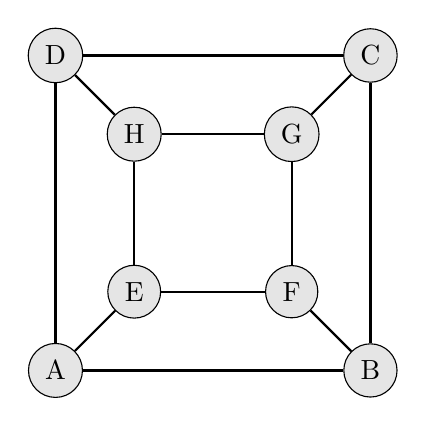
\begin{tikzpicture}
    \node (n1) at (0,0) {D};
    \node (n2) at (4,0) {C};
    \node (n3) at (1,-1) {H};
    \node (n4) at (3,-1) {G};
    \node (n5) at (3,-3) {F};
    \node (n6) at (1,-3) {E};
    \node (n7) at (0,-4) {A};
    \node (n8) at (4,-4) {B};
    \path[draw,thick]
    (n1) edge (n2)
    (n1) edge (n3)
    (n1) edge (n7)
    (n2) edge (n4)
    (n2) edge (n8)
    (n3) edge (n4)
    (n3) edge (n6)
    (n4) edge (n5)
    (n5) edge (n6)
    (n6) edge (n7)
    (n5) edge (n8)
    (n7) edge (n8)
	;
  \end{tikzpicture}
\caption{Graph $F$}
\label{fig:sfig1}
\end{subfigure}
\begin{subfigure}{0.32\textwidth}\centering
  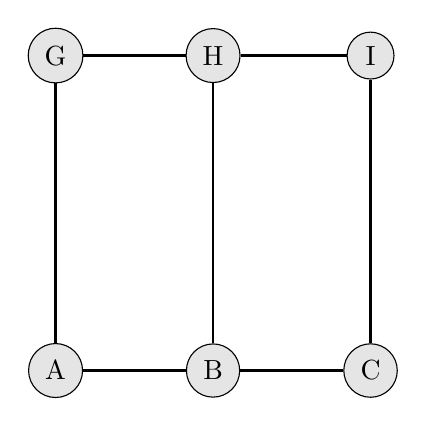
\begin{tikzpicture}
    \node (n1) at (0,0) {A};
    \node (n2) at (2,0) {B};
    \node (n3) at (4,0) {C};
    \node (n4) at (0,4) {G};
    \node (n5) at (2,4) {H};
    \node (n6) at (4,4) {I};
    \path[draw,thick]
    (n1) edge (n2)
    (n2) edge (n3)
    (n4) edge (n5)
    (n5) edge (n6)
    (n1) edge (n4)
    (n2) edge (n5)
    (n3) edge (n6)
	;
  \end{tikzpicture}
\caption{Graph $G$}
\label{fig:sfig2}
\end{subfigure}
\begin{subfigure}{0.32\textwidth}\centering
  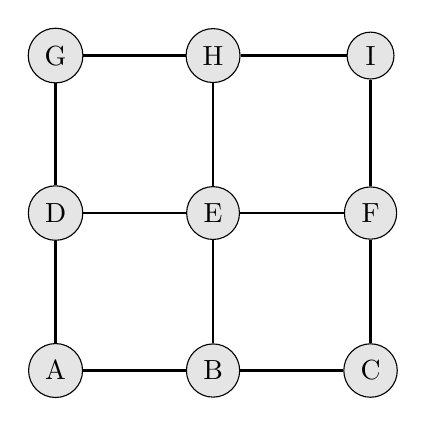
\begin{tikzpicture}
    \node (n1) at (0,0) {A};
    \node (n2) at (2,0) {B};
    \node (n3) at (4,0) {C};
    \node (n4) at (0,2) {D};
    \node (n5) at (2,2) {E};
    \node (n6) at (4,2) {F};
    \node (n7) at (0,4) {G};
    \node (n8) at (2,4) {H};
    \node (n9) at (4,4) {I};
    \path[draw,thick]
    (n1) edge (n2)
    (n2) edge (n3)
    (n4) edge (n5)
    (n5) edge (n6)
    (n7) edge (n8)
    (n8) edge (n9)
    (n1) edge (n4)
    (n2) edge (n5)
    (n3) edge (n6)
    (n4) edge (n7)
    (n5) edge (n8)
    (n6) edge (n9)
	;
  \end{tikzpicture}
\caption{Graph $H$}
\label{fig:sfig3}
\end{subfigure}
\caption{Connected Undirected Graphs for Question 2}\label{fig21}
\end{figure}

\subsection*{Solution}

For a graph $G = (V,E)$ to have a Hamiltonian Cycle, there should be a cycle that contains every vertex in $V$ exactly once.
Therefore, to show a graph $G$ has a Hamiltonian Cycle, it suffices to propose a cycle that begins with $u \in V$, passes every $v \in V-\{u\}$ and ends in $u \in V$.

We can also prove by contradiction that $G$ has a Hamiltonian Cycle $c$ if any vertex $u \in V$ is an endpoint of exactly $2$ edges in $c$.
If $u$ is an endpoint of less than 2 edges, then $u$ is either not connected to $c$ or $c$ is not a cycle; both cases leading to contradiction.
If $u$ is an endpoint of more than two edges, starting from $u$, we can follow $u$ to $v$, using one edge, then return to $u$ using another edge and then visit the third connected vertex.
However, since $c$ is a cycle, we should end our path with $u$, thus visiting $u$ more than twice which contradicts definition of Hamiltonian Cycle.
Therefore, to show that a graph $G$ does not have any Hamiltonian Cycle $c$, we show that there is a vertex $v \in V$ which is an endpoint of more than 2 edges in $c$.
\begin{enumerate}[label=(\alph*)]
\item There is a cycle $c$ of the form $A \rightarrow B \rightarrow C \rightarrow D \rightarrow H \rightarrow G \rightarrow F \rightarrow E \rightarrow A$, that passes through all vertices in $V$ and ends in $A$.
Therefore, Graph $F$ has a Hamiltonian Cycle.
\item There is a cycle $c$ of the form $A \rightarrow B \rightarrow C \rightarrow I \rightarrow H \rightarrow G \rightarrow A$, that passes through all vertices in $V$ and ends in $A$.
Therefore, Graph $G$ has a Hamiltonian Cycle.
\item Vertex $E$ in graph $H$ is connected to $H$ via 4 edges.
Since we proved any Hamiltonian cycle $c$ should pass vertex $E$ with 2 edges, $E$ will be connected to exactly 2 vertices from the set $S = \{B, D, F, H\}$.
Regardless of our choice, choosing any two-element subset of $S$ will immediately divide yet-unvisited vertices into two islands and after visiting one of them, we are unable to visit the other without passing again from an already-visited node.
Therefore, graph $H$ does not have any Hamiltonian Cycle.
\end{enumerate}
